\section{Proposed Methodology}
\title{Proposed Methodology}
\begin{frame}{Proposed Methodology}

% 	\begin{columns}
	    
% 	    \column{.4\textwidth}
    	
%     	\column{.6\textwidth}
    
%     \end{columns}

    \begin{block}{General Concept}
        By the use of the concepts of Information Theory and Bayesian Networks it is intended to unite the method of Transfer Entropy and the K2 algorithm in order to generate a single methodology for the detection of causal relationships.
    \end{block}

    \begin{block}{Approach}
        To model  the system as a graph, in which the nodes will be the entities related to each other, by a causality
        reelationship. This detection will be made in five stages%: Generation of information flow graph, Application of Statistical Threshold, Removal of Cycles, Generation of Common and Virtual Ancestors, Modification and Computation of K2%
    \end{block}
\end{frame}

\begin{frame}{Proposed Methodology}
    \begin{figure}
        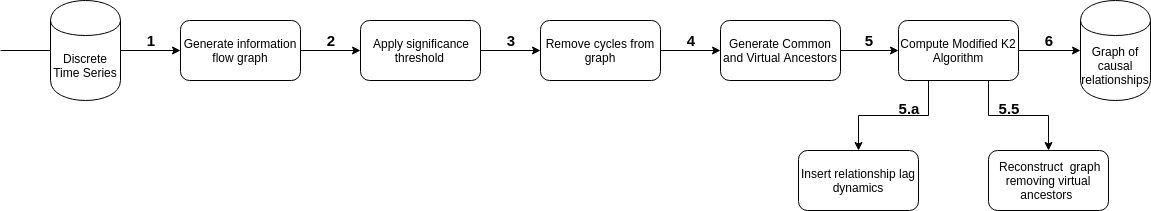
\includegraphics[scale=0.3]{figuras/methodology.png}
        \caption{Proposed Methodology}
    \end{figure}
\end{frame}
\subsection{Generation of graph of information flow}
\begin{frame}{Generation of graph of information flow}

    \begin{columns}
        \column{0.5\textwidth}
            \begin{itemize}
                \item{Given a system with N variables, it computes the Transfer Entropy pairwise for the set of variables.}

                \item{For each pair of variables it computes the method \textit{h} times.}
                
                \item{Chooses the greatest entropy value from the \textit{h} computations.}
            \end{itemize}
        \column{0.5\textwidth}
            \begin{figure}
                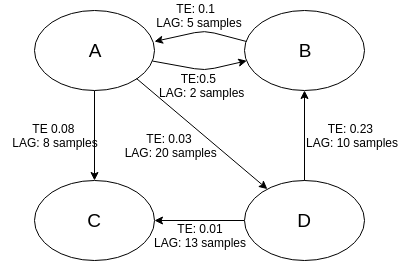
\includegraphics[width=\textwidth]{figuras/graphExample.png}
                \caption{Example of output from stage 1}
            \end{figure}          
    \end{columns}    
\end{frame}


\subsection{Application of Statistical Threshold}
\begin{frame}{Application of Statistical Threshold}

    % \begin{columns}
        % \column{0.5\textwidth}
        \begin{itemize}
            
            \item {  Because the Transfer Entropy is calculated pairwise, it can produce a dense graph. Since due to the noise cointained in the time series,the chance of a zero entopy becames low.
            }
            \item { This stage aims, to the define a threshold for the entropy values based on the distribution of the computed values.}
        \end{itemize}
    
        % \column{0.5\textwidth}

    % \end{columns}
        
\end{frame}

\begin{frame}{Application of Statistical Threshold}
    \begin{figure}
        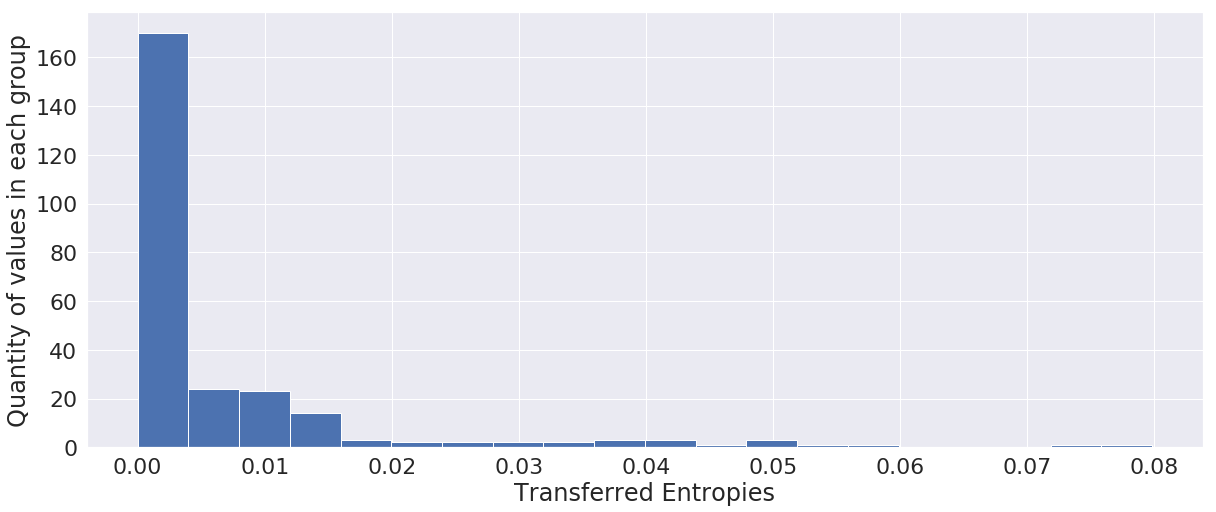
\includegraphics[width=\textwidth]{figuras/hist_ex.png}
    \end{figure}
\end{frame}

\begin{frame}{Application of Statistical Threshold}
    \begin{figure}
        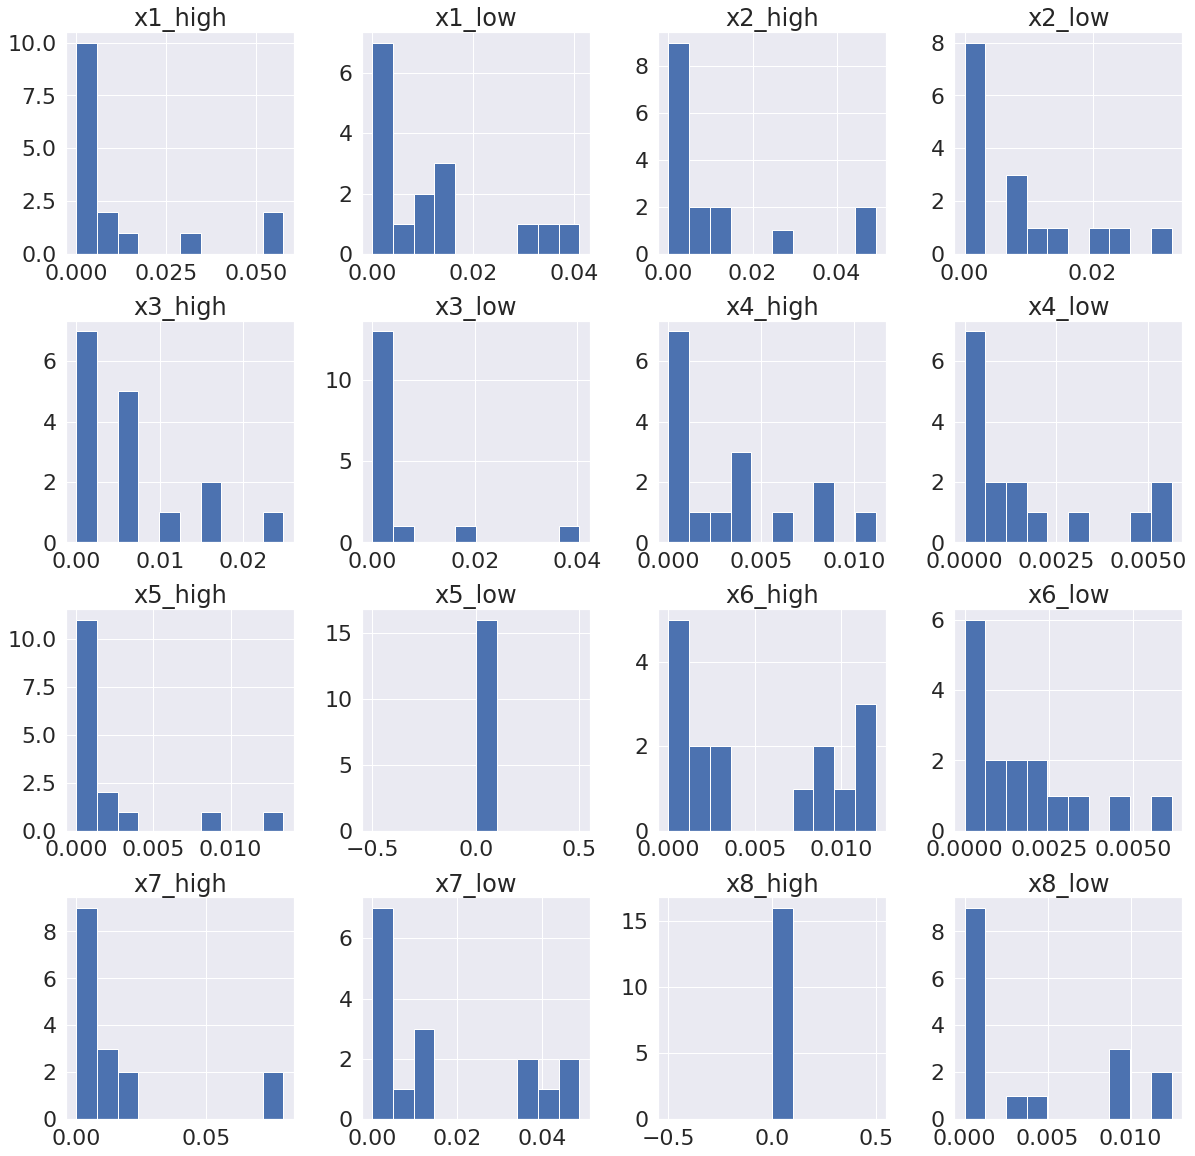
\includegraphics[width=0.8\textwidth, height=60mm]{figuras/mult_hist.png}
    \end{figure}

\end{frame}

\subsection{Removal of Cycles}
\begin{frame}{Removal of Cycles}
    \begin{itemize}
        \item { In order to prepare the graph to be used on K2, third stage does a removal of cycles.}
        \item It consists of recursive search on the graph, in which the nodes “above” the node-cause, are marked as its ancestors. Therefore, he ancestors of a node-cause cannot be related to it as an effect.
        \item {The removal is made based on the criterion of the higher information}
    \end{itemize}

\end{frame}


\begin{frame}{Removal of cycles}
    %Fluxogrma
    
\end{frame}


\subsection{Generation of Common and Virtual Ancestors}
\begin{frame}{Generation of Common and Virtual Ancestors}

\textbf{What is a common and a virtual ancestor?}

\begin{columns}
    \column{0.5\textwidth}
        \begin{figure}
            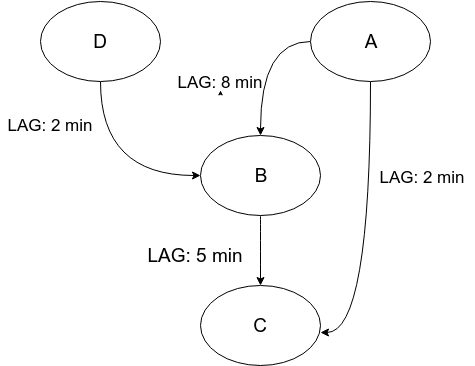
\includegraphics[width=\textwidth]{figuras/virtualNodes.png}
            \caption{Ordinary Graph}
        \end{figure}
    \column{0.5\textwidth}
        \begin{figure}
            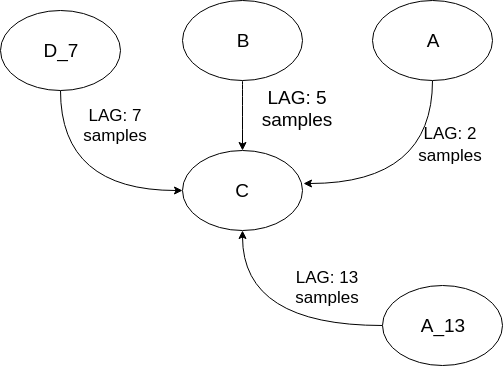
\includegraphics[width=\textwidth]{figuras/cVirt.png}
            \caption{Modified Graph}
        \end{figure}

\end{columns}
\end{frame}

\begin{frame}{Prior Strucuture to K2}
    
\end{frame}

\subsection{Modification and Computation of K2}
\begin{frame}{Modification and Computation of K2}
    
\end{frame}
